\documentclass[UTF8]{article}

\usepackage{amsmath}%数学符号
\usepackage{pgfplots}
\usepackage{enumerate}


\title{Project 5505}
\author{Yifan Li, SImao Gao, Zijian Huang}

\begin{document}

\maketitle

\begin{abstract}
    
    In this project, we analysis the patterns among time of crimes, number of crimes and victims' age and find that 
    
    1. people who are 35 years old are most likely to be attacked. 
    
    2. 7am-8am and 3am-4am is safe time zone comparatively while 4am-6am and 20pm-22pm is the most dangerous. 

    3. The expected number of crimes occurring in one month is among (526.3546, 536.7214).



\end{abstract}


\section{Introduction and Description of Data}

Here are three questions we want to analysis.

\begin{enumerate}
    \item What is the distribution of the age of victims?
    \item Do criminals have a preference for crime time? In other words, is there any association between daily time interval and the number of crime.
    \item What is the distribution of the number of crimes occurring in one month?
\end{enumerate}

Variables we used are: \textit{area.id}, \textit{Date.Occurred}, \textit{Time.Occurred}, and \textit{Victim.Age}.

\section{Exploratory Data Analysis}

\begin{figure}[htb]
    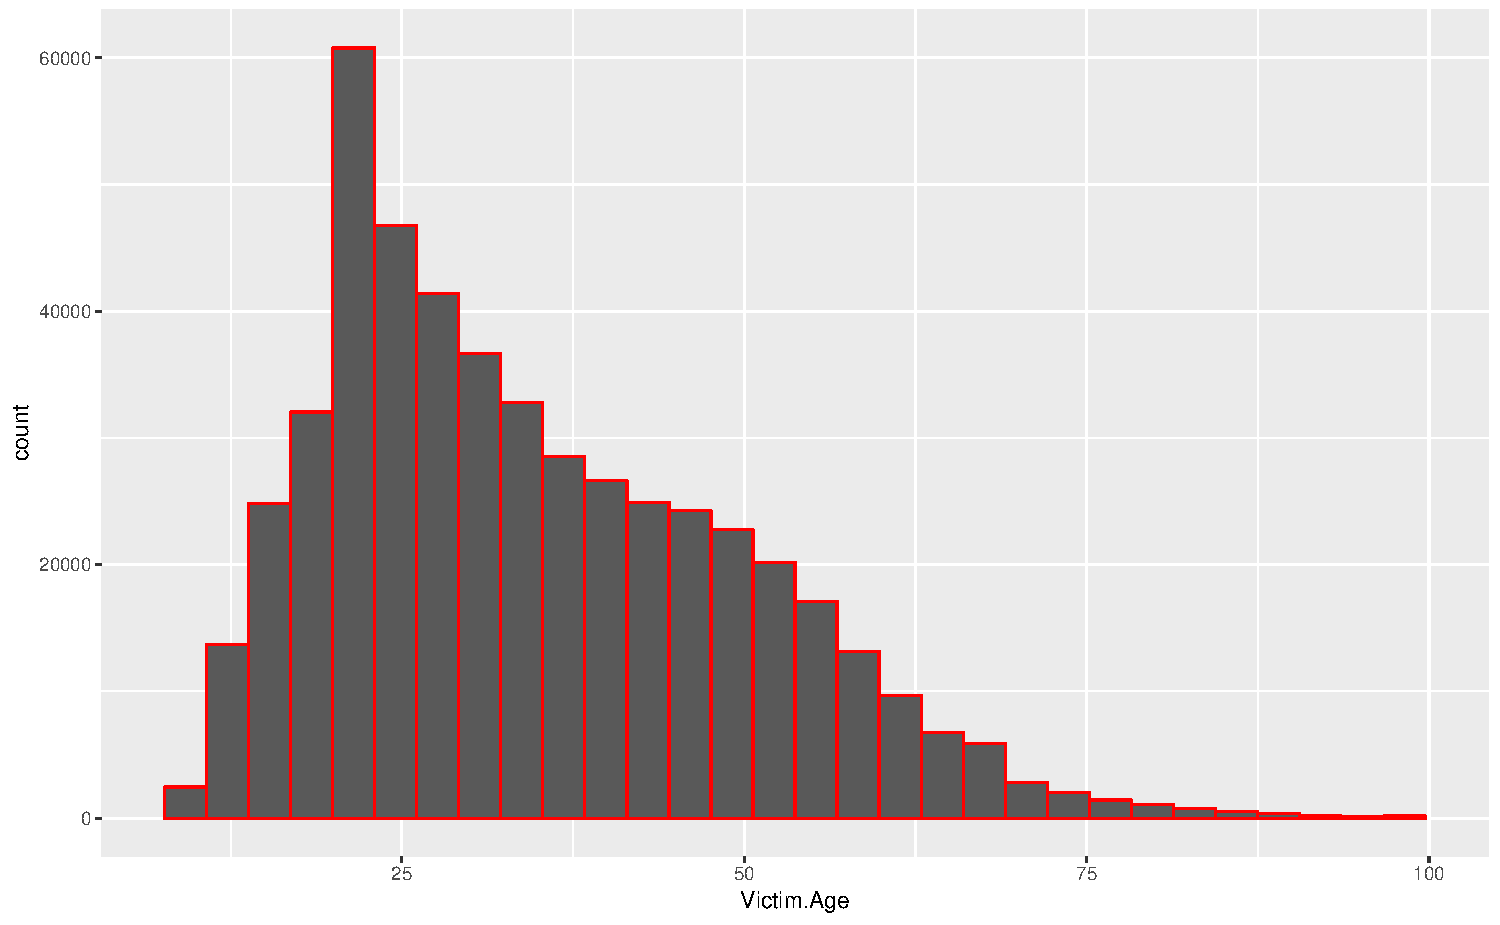
\includegraphics[width=10cm,height=6.18cm]{../image/1.pdf}
    \caption{Histogram of Victim Age}\label{fig:Victim_Age} 
\end{figure}

First we plot the histogram of victims' age. From Figure \ref{fig:Victim_Age}, it is a good idea to fit a poisson distribution.


\newpage

For the purpose to analyze the relationship between the daily time interval with the number of crimes. Firstly, the daily time is cut from 00:00:00 to 24:00:00 into hourly basis, such as, 00:00:00-01:00:00 and 01:00:00-02:00:00. Thus, we will gain 24 intervals. Secondly, the corresponding frequency should be counted. Finally, we plot a histogram of crime in different time intervals.

\begin{figure}[htb]
    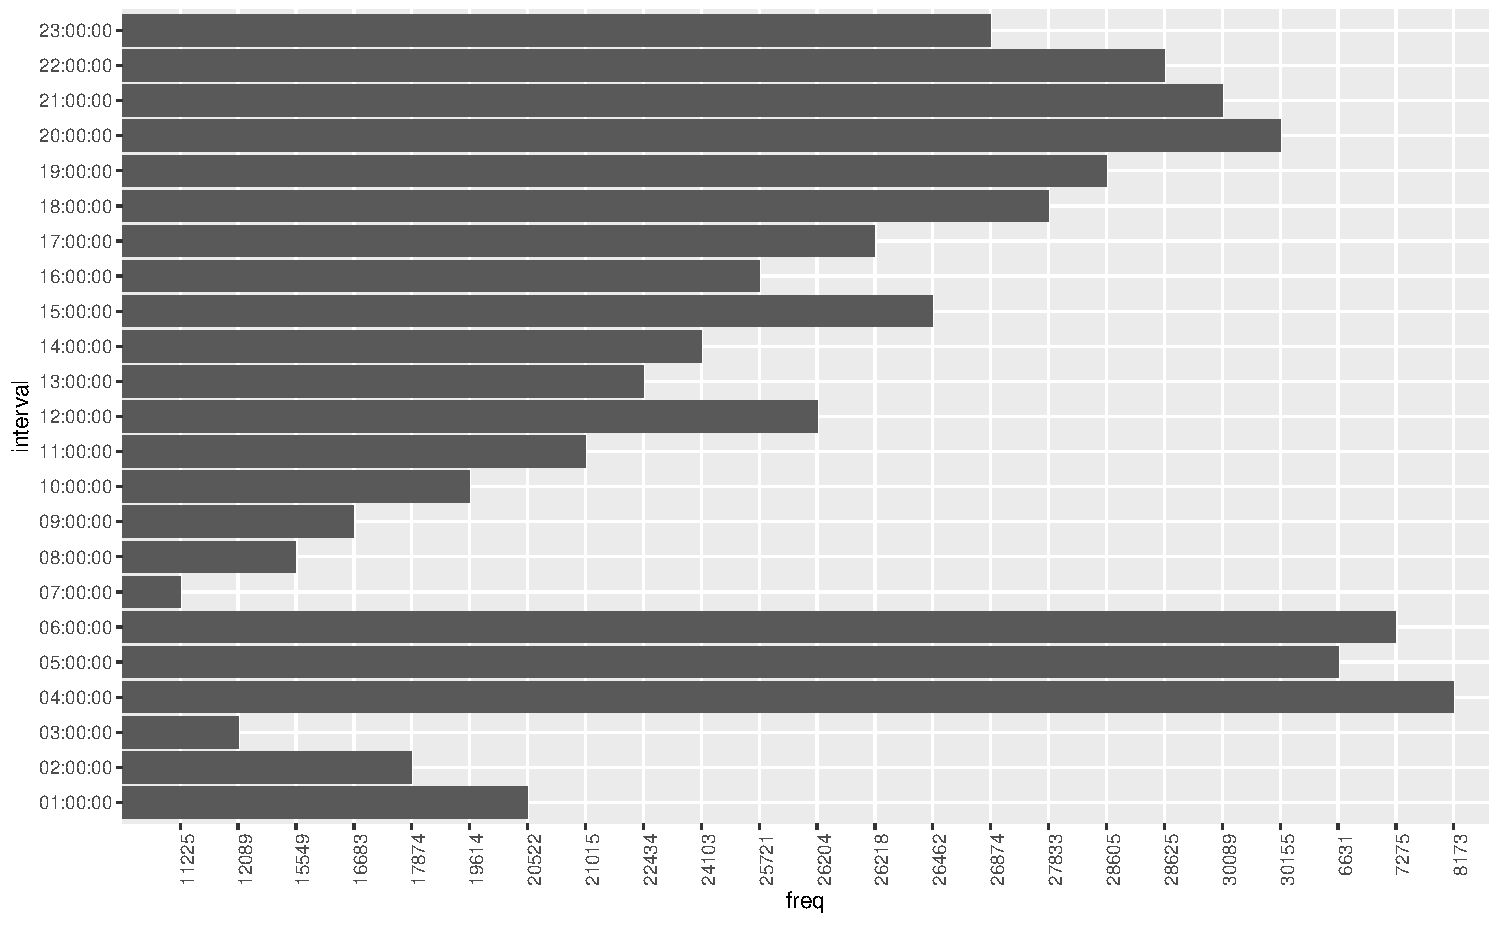
\includegraphics[width=10cm,height=6.18cm]{../image/2.pdf}
    \caption{Histogram of Victim Time}\label{fig:Victim_time} 
\end{figure}

From Figure \ref{fig:Victim_time}, the number of the crime are largest. It also means it will be dangerous during the period during 4am-6am and 20pm-22pm. However, at 7am-8am and 3am-4am will be safe and almost no crime. They may be safe zone.


\section{Statistical Inference}

\subsection{Distribution of the Age of Victims}

\begin{enumerate}[-]
    \item $H_0$: the age of victims follows poisson distribution
    \item Test used: CHi-square test
\end{enumerate}


\begin{figure}[htb]
    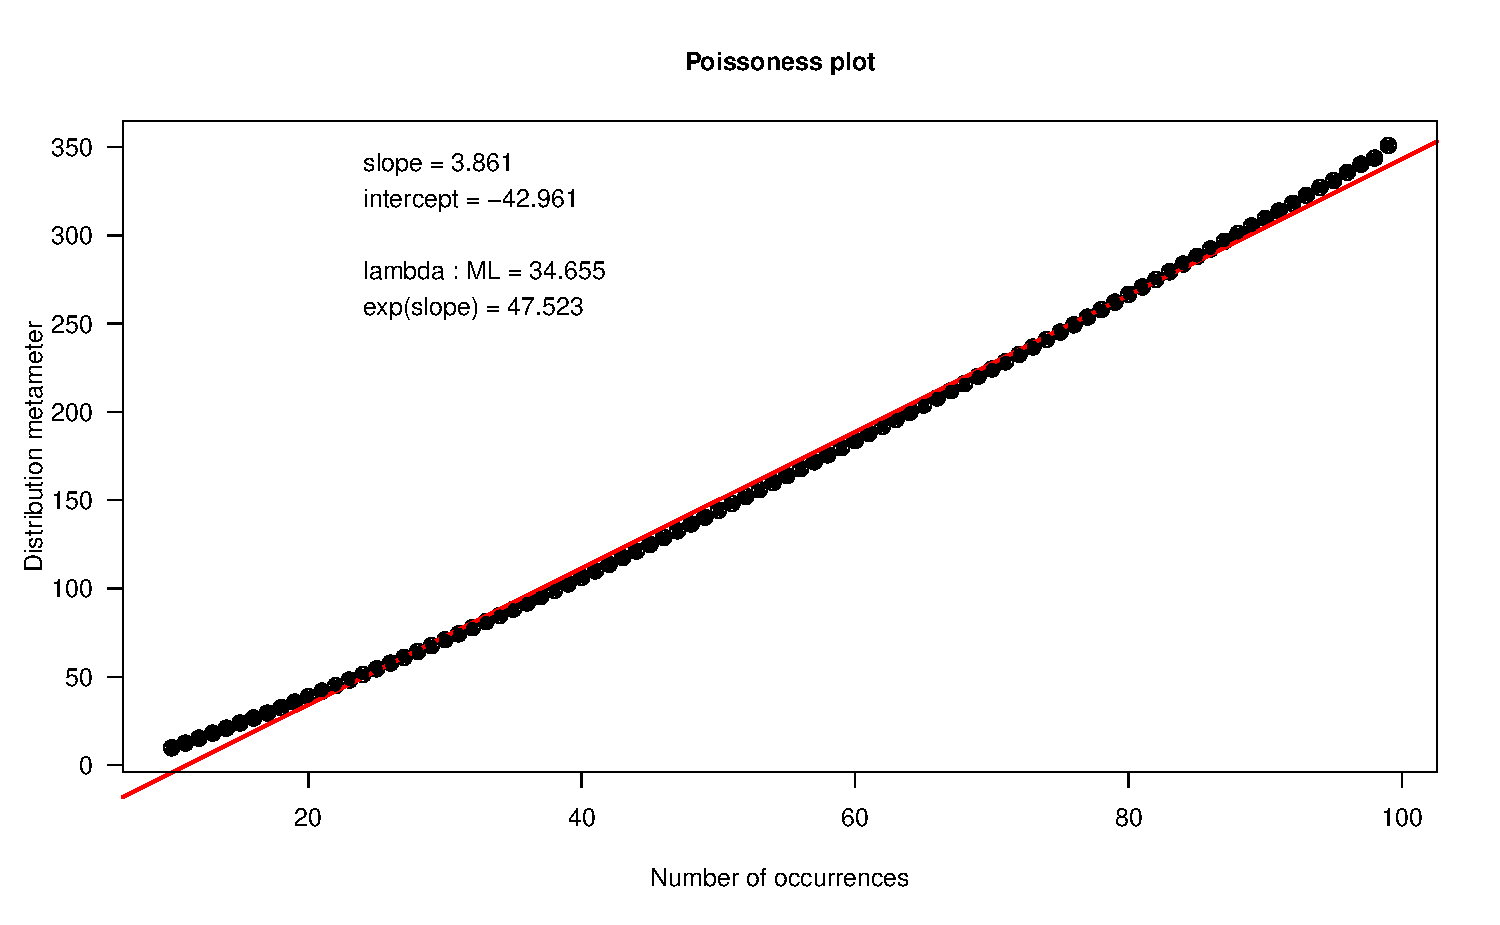
\includegraphics[width=10cm,height=6.18cm]{../image/3.pdf}
    \caption{Poissoness Plot of Victims' Age}\label{fig:poisson_Victim_age} 
\end{figure}

From Figure \ref{fig:poisson_Victim_age}, the poisson distribution fits the data quite well. So we do a Chi-square test to test whether it follows the poisson distribution or not. And the p-value is 0.2492. So we don't reject $H_0$ and the age of victims follows poisson distribution and the MLE estimation of parameter is about 35. This indicates that people who are 35 should be careful. They are most likely to be attacked.

\subsection{Distribution of the Time of Victims}

\begin{enumerate}[-]
    \item $H_0$: the time of victims follows uniform distribution
    \item Test used: CHi-square test
\end{enumerate}

Set the null hypothesis as the frequency follow the union distribution. Actually, from Figure \ref{fig:Victim_time}, the expected result should be not follow the uniform distribution. In other words, there exists relationship between the time interval and frequency. Suppose proportion of the occurrence of each frequency is equal: 1/24= 0.04166667. The expected value of the frequency will be equal to the proportion times the total number of crimes. After apply the chi-square test, we realized that the p-value=0 which will lead us to reject the null hypothesis and state that the distribution of the frequency is not follow uniform distribution. In other words, there exist some relationship between the time interval and frequency.

\subsection{Distribution of the Number of Crimes}

\begin{enumerate}[-]
    \item $H_0$: the number of crimes follows poisson distribution
    \item Test used: Poissoness Plot
\end{enumerate}

\begin{figure}[htb]
    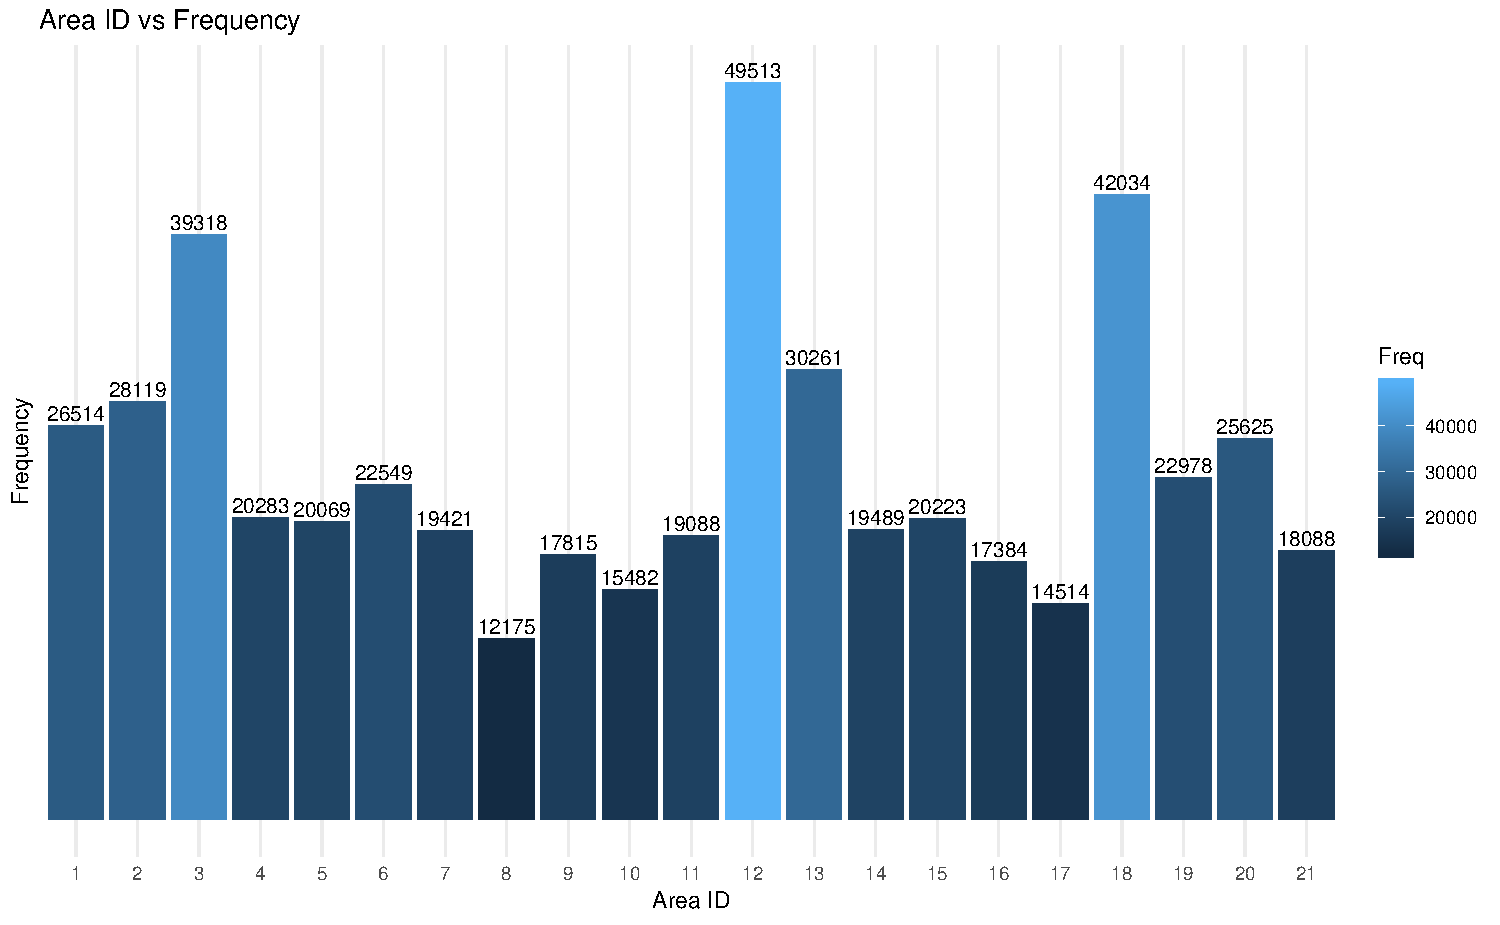
\includegraphics[width=10cm,height=6.18cm]{../image/4.pdf}
    \caption{Area ID vs Frequency}\label{fig:Frequency} 
\end{figure}

From Figure \ref{fig:Frequency}, area with id “12” has the highest frequency of crimes. So we are curious that whether the number of crimes occurrence in each month for area 12 follows distribution or not, hence, we construct poissonness plot to find out.

\begin{figure}[htb]
    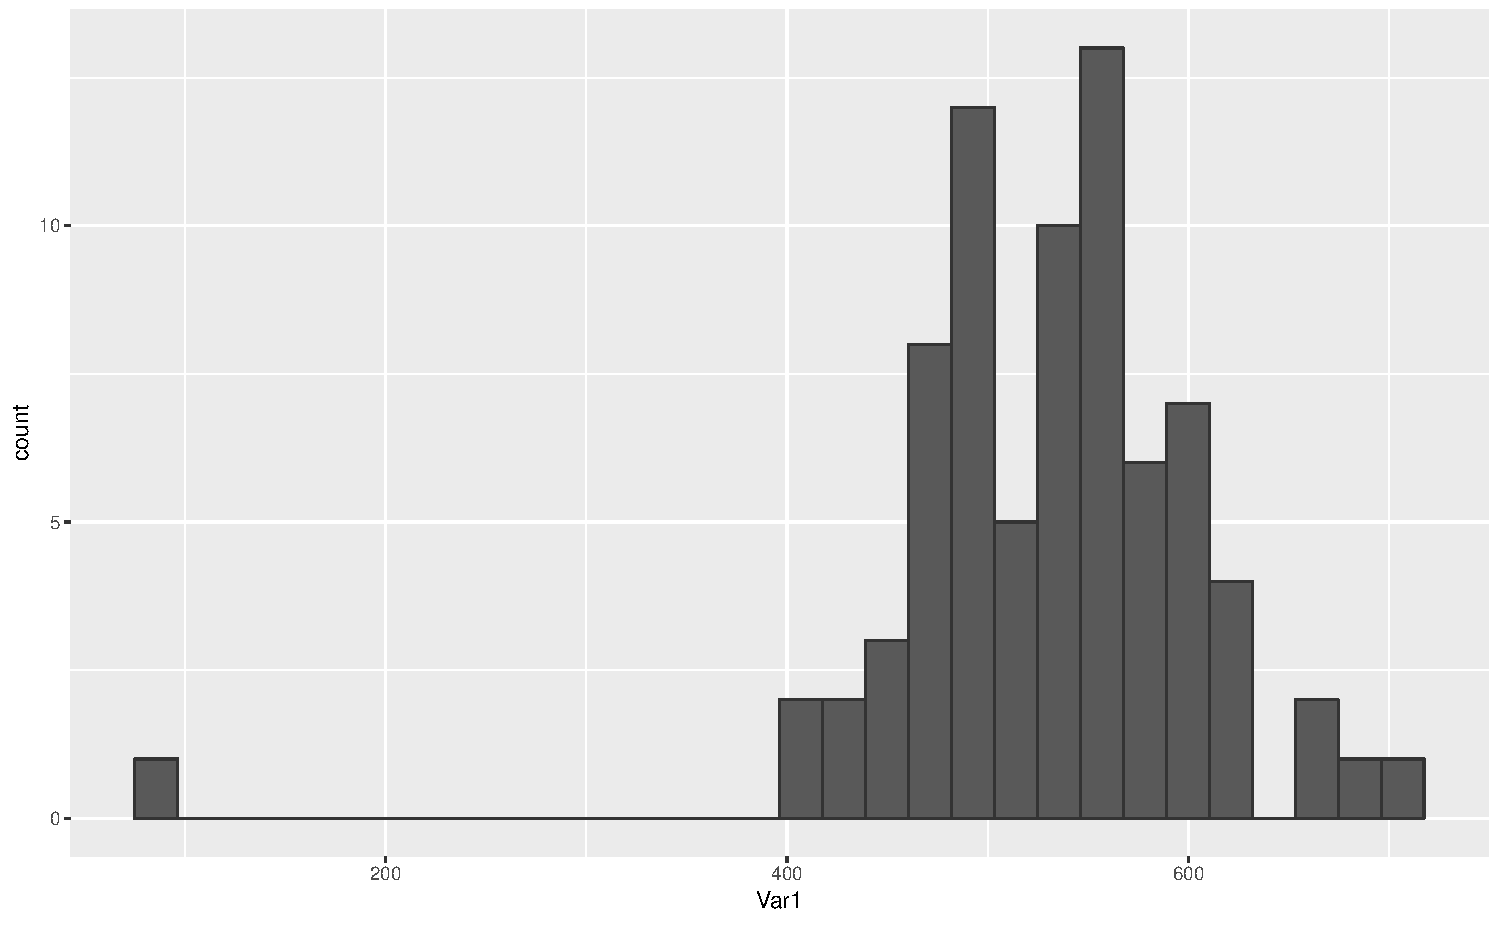
\includegraphics[width=7cm,height=4cm]{../image/5.pdf}
    \caption{Histogram of Crimes' number}\label{fig:outliar} 
\end{figure}


From Figure \ref{fig:outliar}, “2017-10” is a outlier since it has only 80 crimes comparing to 500-800 crimes for other months. After removing the outlier, the poissoness plot is as follows.


\begin{figure}[htb]
    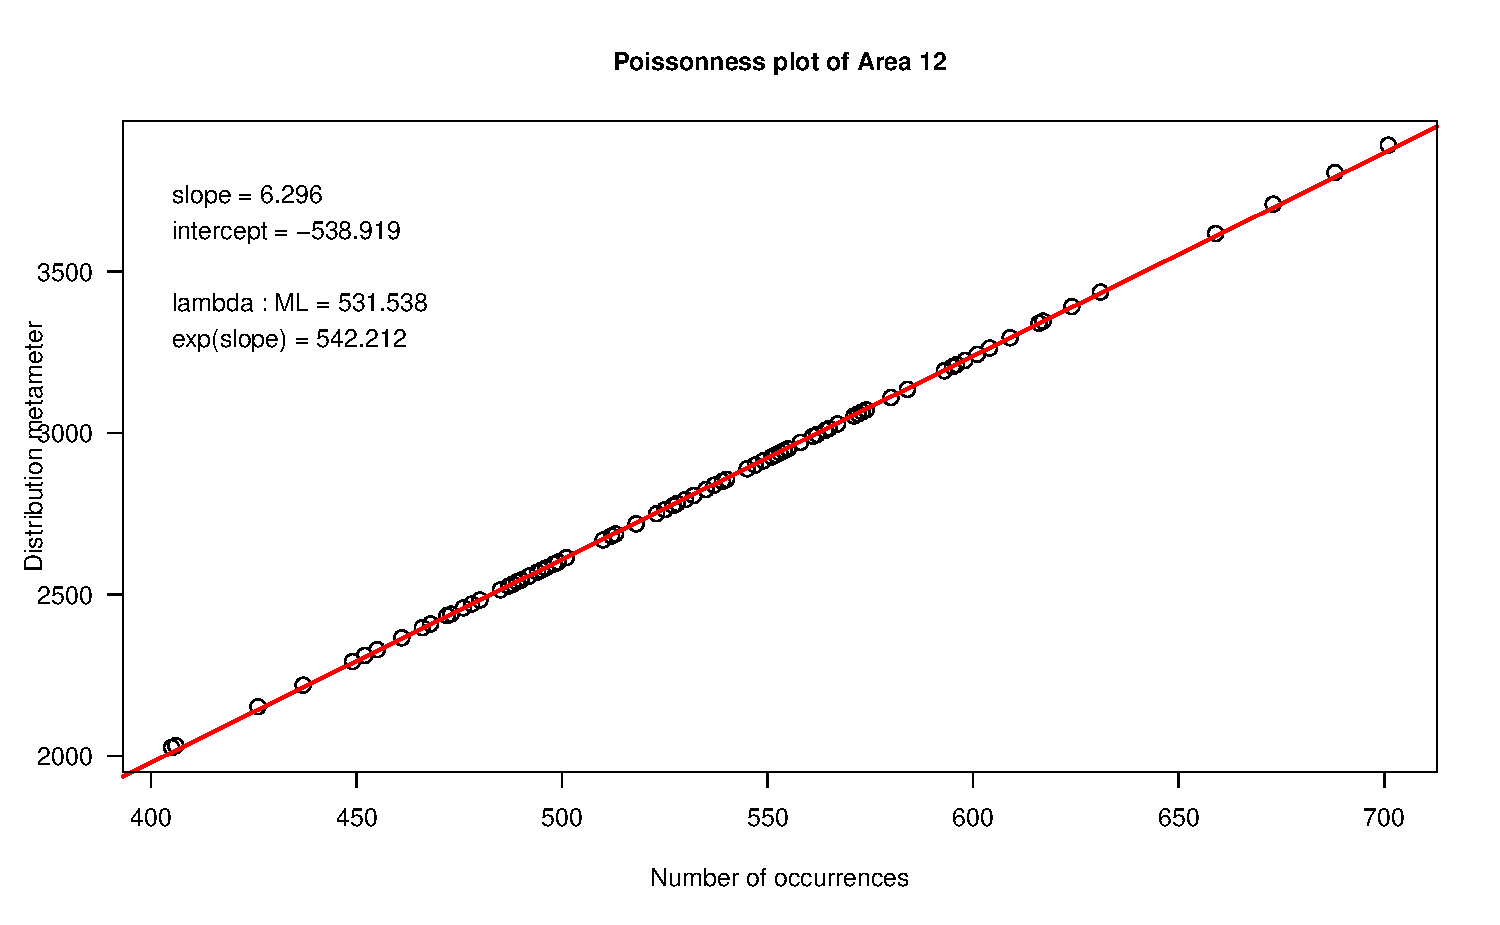
\includegraphics[width=10cm,height=6.18cm]{../image/6.pdf}
    \caption{Poissoness Plot of Crimes' number}\label{fig:poisson_Crime_number} 
\end{figure}


From Figure \ref{fig:poisson_Crime_number}, it is apparent that the points approximated lay on the straight line. We can say that poisson distribution fits the data set.

Therefore, with MLE of $\lambda$, we can calculate the 95\% confidence interval for this MLE. $Var(\hat{\lambda})=\sqrt{\frac{\hat{\lambda}}{n}}$.Therefore, the 95\% confidence interval for $\lambda$ using MLE method is (526.3546, 536.7214). 



\section{Conclusion}

So, our conclusion is:

\begin{enumerate}
    \item The age of victims follow a poisson distribution with parameter equal to 35.
    \item There exists association between daily time interval and the number of crime.
    \item The number of crimes occurring in one month follows poisson distribution. 95\% confidence interval for it is (526.3546, 536.7214).
\end{enumerate}


\end{document}  